% Author: Izaak Neutelings (February 2020)
% from https://tikz.net/capacitors/
\documentclass[border=3pt,tikz]{standalone}
\usepackage{amsmath} % for \dfrac
\usepackage{bm}
\usepackage{physics}
\usepackage{tikz,pgfplots}
\usetikzlibrary{angles,quotes} % for pic (angle labels)
\usetikzlibrary{decorations.markings}
\usetikzlibrary{calc}
\usetikzlibrary{shapes,intersections} % for path name
\tikzset{>=latex} % for LaTeX arrow head

\usepackage{xcolor}
\colorlet{Ecol}{orange!90!black}
\colorlet{EcolFL}{orange!90!black}
\colorlet{veccol}{green!45!black}
\colorlet{EFcol}{red!60!black}
\colorlet{pluscol}{red!60!black}
\colorlet{minuscol}{blue!60!black}
\tikzstyle{anode}=[top color=red!20,bottom color=red!50,shading angle=20]
\tikzstyle{cathode}=[top color=blue!20,bottom color=blue!40,shading angle=20]
\tikzstyle{charge+}=[very thin,top color=red!80,bottom color=red!80!black,shading angle=-5]
\tikzstyle{charge-}=[very thin,top color=blue!50,bottom color=blue!70!white!90!black,shading angle=10]
\tikzstyle{vector}=[->,thick,veccol]
\tikzstyle{normalvec}=[->,thick,blue!80!black!80]
\tikzstyle{Cstyle}=[very thick,orange!90!black]
\tikzstyle{EField}=[->,thick,Ecol]
\tikzstyle{EField dashed}=[dashed,Ecol,line width=0.6]
\tikzset{
  EFieldLine/.style={thick,EcolFL,decoration={markings,
                     mark=at position #1 with {\arrow{latex}}},
                     postaction={decorate}},
  EFieldLine/.default=0.5}
\tikzstyle{measure}=[fill=white,midway,outer sep=2]

\def\dpa{0.28}
\def\dba{0.14}
\def\dipole#1#2{
  \begin{scope}[shift={(#1)},rotate=#2]
    \draw[charge-] (-\dpa,0) to[out=90,in=180] (0,\dba) -- (0,-\dba) to[out=180,in=-90] cycle;
    \draw[charge+] ( \dpa,0) to[out=90,in=  0] (0,\dba) -- (0,-\dba) to[out=  0,in=-90] cycle;
    \node[scale=0.7] at (-\dpa/2,0) {$-$};
    \node[scale=0.7] at ( \dpa/2,0) {$+$};
  \end{scope}
}

\begin{document}


% CAPACITOR 3D
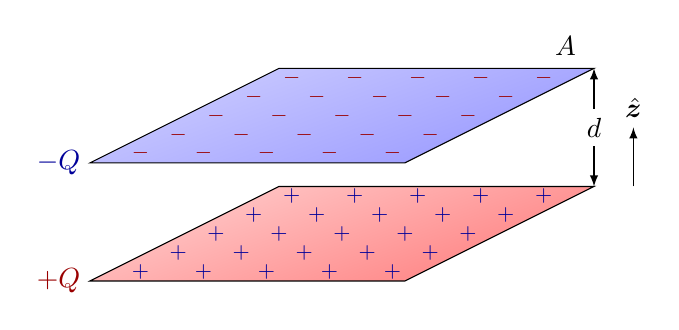
\begin{tikzpicture}[x={(1cm,0)},y={(0.6cm,0.3cm)},z={(0,1cm)}]
  \def\H{1.5}
  \def\W{4}
  \def\L{4}
  \def\Nx{5}
  \def\Ny{5}
  \draw[anode]
    (0,0,0) --++ (\L,0,0) --++ (0,\W,0) --++ (-\L,0,0) -- cycle;
  \draw[cathode]
    (0,0,\H) --++ (\L,0,0) --++ (0,\W,0) --++ (-\L,0,0) -- cycle;
  \foreach \i [evaluate={\x=(\i-0.5)*\L/\Nx;}] in {1,...,\Nx}{
    \foreach \j [evaluate={\y=(\j-0.5)*\W/\Ny;}] in {1,...,\Ny}{
      \node[minuscol,scale=0.8] at (\x,\y,0) {$+$};
      \node[pluscol,scale=0.8] at (\x,\y,\H) {$-$};
    }
  }
  \node[pluscol,left] at (0,0,0) {$+Q$};
  \node[minuscol,left] at (0,0,\H) {$-Q$};
  \node[left=2,above left=1] at (\L,\W,\H) {$A$};
  \draw[<->] (\L,\W,0) -- (\L,\W,\H) node[measure] {$d$};
  \draw[-{latex}] (\L + 0.5,\W,0) -- (\L+0.5,\W, {0.5*\H}) node[above] {$\hat{\boldsymbol{z}}$};
\end{tikzpicture}


% CAPACITOR 2D
\def\H{4.5}
\def\W{3.0}
\def\w{0.4}
\def\a{0.15*\W}
\def\NE{6}
\def\NQ{7}
\begin{tikzpicture}
  
  % ELECTRIC FIELD
  \foreach \i [evaluate={\y=(\i-0.75)*\H/(\NE-0.5);}] in {1,...,\NE}{
    \draw[EFieldLine={0.54},very thick] (0,\y) --++ (\W,0);
  }
  
  % PLATES
  \draw[anode]
    (0,0) rectangle++ (-\w,\H);
  \draw[cathode]
    (\W,0) rectangle++ (\w,\H);
  \foreach \i [evaluate={\y=(\i-0.5)*\H/\NQ;}] in {1,...,\NQ}{
    \node[pluscol,scale=0.9] at (-\w/2,\y) {$+$};
    \node[minuscol,scale=0.9] at (\W+\w/2,\y) {$-$};
  }
  \node[Ecol,above] at (0.48*\W,1.0*\H) {$\vb{E}$};
  \node[pluscol] at (-2.1*\w,\H) {$+Q$};
  \node[minuscol] at (\W+2.1*\w,\H) {$-Q$};
  \draw[very thin] (0.005,-0.04*\H) --++ (0,0.05*\H);
  \draw[very thin] (\W-0.005,-0.04*\H) --++ (0,0.05*\H);
  \draw[<->] (0.005,-0.02*\H) --++ (\W-0.01,0) node[measure,inner sep=2] {$d$};
  
\end{tikzpicture}


% CAPACITOR 2D - realistic
\begin{tikzpicture}
  \def\NE{4}
  \def\R{2.5}
  
  % ELECTRIC FIELD
  \foreach \i [evaluate={\y=0.55*(\i-0.5)*\H/\NE; \ang=(\i-1)*(\i-1)*20/\NE;}] in {1,...,\NE}{
    \draw[EFieldLine={0.52},very thick] (0,\H/2+\y) to[out=\ang,in=180-\ang]++ (\W,0);
    \draw[EFieldLine={0.52},very thick] (0,\H/2-\y) to[out=-\ang,in=180+\ang]++ (\W,0);
  }
  \foreach \y/\ang/\out/\in in {0.8/60/20/-100,0.45/30/5/-120}{
    \draw[EFieldLine={0.6},very thick] (\W+\w,{(1+\y)*\H/2})++(\ang:\R) to[out=\in,in=\out]++ (\ang:-\R);
    \draw[EFieldLine={0.6},very thick] (\W+\w,{(1-\y)*\H/2})++(-\ang:\R) to[out=-\in,in=-\out]++ (-\ang:-\R);
    \draw[EFieldLine={0.6},very thick] (-\w,{(1+\y)*\H/2}) to[out=180-\out,in=180-\in]++ (-\ang:-\R);
    \draw[EFieldLine={0.6},very thick] (-\w,{(1-\y)*\H/2}) to[out=180+\out,in=180+\in]++ (+\ang:-\R);
  }
  \draw[EFieldLine={0.52},very thick] (-0.9*\w,\H) to[out=110,in=70,looseness=1.8] (\W+0.9*\w,\H);
  \draw[EFieldLine={0.52},very thick] (-0.9*\w,0) to[out=-110,in=-70,looseness=1.8] (\W+0.9*\w,0);
  \draw[EFieldLine={0.65},very thick] (\W+\w+0.9*\R,\H/2) --++ (-0.9*\R,0);
  \draw[EFieldLine={0.65},very thick] (-\w,\H/2) --++ (-0.9*\R,0);
  
  % PLATES
  \draw[anode]
    (0,0) rectangle++ (-\w,\H);
  \draw[cathode]
    (\W,0) rectangle++ (\w,\H);
  \foreach \i [evaluate={\y=(\i-0.5)*\H/\NQ;}] in {1,...,\NQ}{
    \node[pluscol,scale=0.9] at (-\w/2,\y) {$+$};
    \node[minuscol,scale=0.9] at (\W+\w/2,\y) {$-$};
  }
  %\node[Ecol,above] at (0.48*\W,1.0*\H) {$\vb{E}$};
  
\end{tikzpicture}


% DIPOLES without capacitors
\begin{tikzpicture}
  
  % DIELECTRIC
  \draw[orange!60!black,fill=orange!80!brown!5]
    (\a,-0.03*\H) rectangle (\W-\a,1.03*\H);
    
  % DIPOLE
  \dipole{0.26*\W,0.1*\H}{320}
  \dipole{0.26*\W,0.3*\H}{220}
  \dipole{0.26*\W,0.5*\H}{30}
  \dipole{0.26*\W,0.7*\H}{260}
  \dipole{0.26*\W,0.9*\H}{70}
  \dipole{0.50*\W,0.1*\H}{30}
  \dipole{0.50*\W,0.3*\H}{160}
  \dipole{0.50*\W,0.5*\H}{80}
  \dipole{0.50*\W,0.7*\H}{150}
  \dipole{0.50*\W,0.9*\H}{110}
  \dipole{0.74*\W,0.1*\H}{100}
  \dipole{0.74*\W,0.3*\H}{220}
  \dipole{0.74*\W,0.5*\H}{160}
  \dipole{0.74*\W,0.7*\H}{30}
  \dipole{0.74*\W,0.9*\H}{340}
  
\end{tikzpicture}


% CAPACITOR 2D - dipole
\begin{tikzpicture}
  
  % DIELECTRIC
  \draw[orange!60!black,fill=orange!80!brown!5]
    (\a,-0.03*\H) rectangle (\W-\a,1.03*\H);
  
  % ELECTRIC FIELD
  \foreach \i [evaluate={\y=(\i-0.75)*\H/(\NE-0.5);}] in {1,...,\NE}{
    \draw[EFieldLine={0.54},very thick] (0,\y) --++ (\W,0);
  }
  
  % PLATES
  \draw[anode]
    (0,0) rectangle++ (-\w,\H);
  \draw[cathode]
    (\W,0) rectangle++ (\w,\H);
  \foreach \i [evaluate={\y=(\i-0.5)*\H/\NQ;}] in {1,...,\NQ}{
    \node[pluscol,scale=0.9] at (-\w/2,\y) {$+$};
    \node[minuscol,scale=0.9] at (\W+\w/2,\y) {$-$};
  }
  \node[Ecol,above] at (0.48*\W,1.05*\H) {$\vb{E}$};
  \node[above,scale=0.95,minuscol] at (   1.3*\a,1.02*\H) {$-\sigma_\mathrm{b}$};
  \node[above,scale=0.95,pluscol]  at (\W-1.3*\a,1.02*\H) {$+\sigma_\mathrm{b}$};
  \node[above,scale=0.95,pluscol]  at (  -0.5*\w,0.99*\H) {$+\sigma_\mathrm{f}$};
  \node[above,scale=0.95,minuscol] at (\W+0.5*\w,0.99*\H) {$-\sigma_\mathrm{f}$};
  
  % DIPOLE
  \dipole{0.26*\W,0.1*\H}{0}
  \dipole{0.26*\W,0.3*\H}{0}
  \dipole{0.26*\W,0.5*\H}{0}
  \dipole{0.26*\W,0.7*\H}{0}
  \dipole{0.26*\W,0.9*\H}{0}
  \dipole{0.50*\W,0.1*\H}{0}
  \dipole{0.50*\W,0.3*\H}{0}
  \dipole{0.50*\W,0.5*\H}{0}
  \dipole{0.50*\W,0.7*\H}{0}
  \dipole{0.50*\W,0.9*\H}{0}
  \dipole{0.74*\W,0.1*\H}{0}
  \dipole{0.74*\W,0.3*\H}{0}
  \dipole{0.74*\W,0.5*\H}{0}
  \dipole{0.74*\W,0.7*\H}{0}
  \dipole{0.74*\W,0.9*\H}{0}
  
\end{tikzpicture}


% CAPACITOR 2D - dielectric
\begin{tikzpicture}
  
  % DIELECTRIC
  \draw[orange!60!black,fill=orange!80!brown!45]
    (\a,-0.03*\H) rectangle (\W-\a,1.03*\H);
  
  % ELECTRIC FIELD
  \foreach \i [evaluate={\y=(\i-0.75)*\H/(\NE-0.5);}] in {1,...,\NE}{
    \draw[EFieldLine={0.54},very thick] (0,\y) --++ (\W,0);
  }
  
  % PLATES
  \draw[anode]
    (0,0) rectangle++ (-\w,\H);
  \draw[cathode]
    (\W,0) rectangle++ (\w,\H);
  \foreach \i [evaluate={\y=(\i-0.5)*\H/\NQ;}] in {1,...,\NQ}{
    \node[pluscol,scale=0.9] at (-\w/2,\y) {$+$};
    \node[minuscol,scale=0.9] at (\W+\w/2,\y) {$-$};
  }
  \node[Ecol,above] at (0.48*\W,1.05*\H) {$\vb{E}$};
  
\end{tikzpicture}


% CAPACITOR 2D - dielectric force
\begin{tikzpicture}
  \def\H{6.4}
  \def\W{2.0}
  \def\w{0.4}
  \def\NE{5}
  \def\NQ{8}
  
  % DIELECTRIC
  \draw[orange!60!black,fill=orange!80!brown!45]
    (0.46*\H,\a) rectangle ++(\H,\W-2*\a);
  \foreach \i [evaluate={\x=0.46*\H+(\i-0.5)*\H/\NQ;}] in {1,...,\NQ}{
    \node[red!60!black,scale=0.9,below] at (\x,\W-\a) {$+$};
    \node[blue!60!black,scale=0.9,above] at (\x,\a) {$-$};
  }
  \draw[->,EFcol,very thick]
    (0.46*\H,\W/2) --++ (-0.15*\H,0) node[right=2,above=2] {$\vb{F}$};
  \draw[->,thick]
    (1.1*\H,-\w/2) --++ (0.2*\H,0) node[right=2] {$x$};
  
  % ELECTRIC FIELD
  \foreach \i [evaluate={\x=(\i-0.75)*\H/(\NE-0.5);}] in {1,...,\NE}{
    \draw[EFieldLine={0.57},very thick] (\x,0) --++ (0,\W);
  }
  
  % PLATES
  \draw[anode]
    (0,0) rectangle++ (\H,-\w);
  \draw[cathode]
    (0,\W) rectangle++ (\H,\w);
  \foreach \i [evaluate={\x=(\i-0.5)*\H/\NQ;}] in {1,...,\NQ}{
    \node[pluscol,scale=0.9] at (\x,-\w/2) {$+$};
    \node[minuscol,scale=0.9] at (\x,\W+\w/2) {$-$};
  }
  \node[Ecol] at (-0.01*\H,\W/2) {$\vb{E}$};
  
\end{tikzpicture}


% CAPACITOR 2D - circular
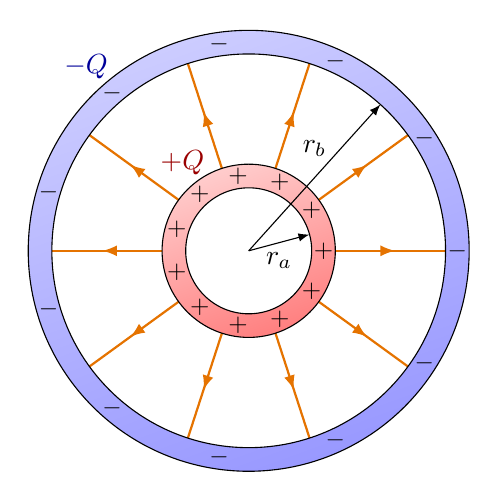
\begin{tikzpicture}
  \def\NE{10}
  \def\NQ{11}
  \def\Rin{0.8}
  \def\Rout{2.5}
  \def\a{0.3}
  
  % ELECTRIC FIELD
  \foreach \i [evaluate={\ang=\i*360/\NE;}] in {1,...,\NE}{
    \draw[EFieldLine={0.54},thick] (\ang:\Rin+\a) -- (\ang:\Rout);
  }
  
  % PLATES
  \draw[anode,even odd rule]
    (0,0) circle (\Rin) circle (\Rin+\a);
  \draw[cathode,even odd rule]
    (0,0) circle (\Rout) circle (\Rout+\a);
  \foreach \i [evaluate={\ang=\i*360/\NQ;}] in {1,...,\NQ}{
    \node[scale=0.9] at (\ang:\Rin+\a/2) {$+$};
    \node[scale=0.9] at (\ang:\Rout+\a/2) {$-$};
  }
  \node[pluscol,above] at (135:\Rin+1.3*\a) {$+Q$};
  \node[minuscol,above] at (135:\Rout+1.4*\a) {$-Q$};
  %\node[Ecol,above] at (0.48*\W,1.05*\H) {$\vb{E}$};
  \draw[->] (0,0) -- (15:\Rin) node[midway,below] {$r_a$};
  \draw[->] (0,0) -- (48:\Rout) node[midway,above=4] {$r_b$};
  
\end{tikzpicture}


% CAPACITOR
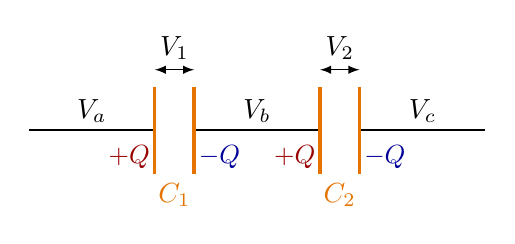
\begin{tikzpicture}
  \def\h{1.1}
  \def\l{1.6}
  \def\g{0.5}
  %\hnode[pluscol,above] at (135:\Rin+1.3*\l) {$+Q$};
  \draw[thick] (0,0) -- (\l,0) coordinate (C1L) node[midway,above=-1] {$V_a$};
  \draw[thick] (C1L)++(\g,0) coordinate (C1R) --++ (\l,0) coordinate (C2L) node[midway,above=-1] {$V_b$};
  \draw[thick] (C2L)++(\g,0) coordinate (C2R) --++ (\l,0) node[midway,above=-1] {$V_c$};
  \draw[Cstyle] (C1L)++(0,-\h/2) node[pluscol, above left=-2, scale=0.95] {$+Q$} --++ (0,\h) coordinate (C1LT);
  \draw[Cstyle] (C1R)++(0,-\h/2) node[minuscol,above right=-2,scale=0.95] {$-Q$} --++ (0,\h) coordinate (C1RT);
  \draw[Cstyle] (C2L)++(0,-\h/2) node[pluscol, above left=-2, scale=0.95] {$+Q$} --++ (0,\h) coordinate (C2LT);
  \draw[Cstyle] (C2R)++(0,-\h/2) node[minuscol,above right=-2,scale=0.95] {$-Q$} --++ (0,\h) coordinate (C2RT);
  \draw[<->] ($(C1LT)+(0,0.2*\h)$) -- ($(C1RT.90)+(0,0.2*\h)$) node[midway,above] {$V_1$};
  \draw[<->] ($(C2LT)+(0,0.2*\h)$) -- ($(C2RT.90)+(0,0.2*\h)$) node[midway,above] {$V_2$};
  \node[Ecol,below] at ($(C1L)+(\g/2,-\h/2)$) {$C_1$};
  \node[Ecol,below] at ($(C2L)+(\g/2,-\h/2)$) {$C_2$};
\end{tikzpicture}


\end{document}